\chapter{Specifikace cílů práce}

Účelem této sekce je stanovení přesného popisu řešené problematiky a cílů práce. Tyto cíle popíšeme formou požadavků na výsledky práce. Při specifikaci požadavků budeme vycházet ze zadání. Na základě zadání můžeme specifikovat tři oblasti požadavků.

V~první oblasti se budeme zabývat požadavky na rešeršní části práce -- analýzu \emph{principů} používaných při \emph{objektově orientovaném návrhu a implementaci}. Část druhá bude obsahovat požadavky na \emph{formalizaci pravidel}, která umožní popsat principy analyzované v~části první. Třetí část poskytne rozbor \emph{požadavků na systém}, který by měl demonstrovat vyhodnocování/validaci definovaných pravidel na existujících zdrojových kódech.

Na konci kapitoly rozebereme v~rámci jedné sekce existující podobná řešení/nástroje, jejich výhody a nevýhody.

\section{Požadavky na analýzu základních návrhových principů}
\label{requirements-principle_analysis}
Zadání práce specifikuje konkrétně tři návrhové principy -- \emph{low coupling}, \emph{high cohesion} a \emph{Law of Demeter}. Tyto principy jsou si v~mnohém podobné. Všechny se zabývají zejména závislostmi mezi částmi zdrojových kódů a jejich propojeností.

V~části analýzy je nutné projít postupně tyto návrhové principy a určit jejich vlastnosti a možnosti ověřování. To zahrnuje zejména provedení rešerší a specifikaci konkrétních tvrzení, která bude následně možné převést na pravidla. Může se ukázat, že ne všechny principy jsou exaktně definované, ověřitelné a vynutitelné. V~takových případech je možné uvažovat spíše statistický přístup oproti ověřování pravidel. Výsledkem by potom nebyl výsledek splňuje/nesplňuje, ale např. množina statistických atributů (features), na níž by bylo možné provádět další druhy analýzy (klasifikaci, pattern matching, \ldots).

Výsledkem analýzy principů by mělo být především vymezení oblasti, kterou se budeme zabývat v~další části -- \emph{formalizaci pravidel}.

\section{Požadavky na formalizaci pravidel}

Formalizace pravidel bude mít dvě hlavní součásti. V~obecné části bude definován model nad nímž budeme stavět pravidla a formát/způsob zápisu pravidel. Konkrétní část potom poskytne specifikaci pravidel \emph{Law of Demeter}, \emph{low coupling} a \emph{high cohesion} v~navrženém formalismu (bude-li to možné).

Definice modelu bude zahrnovat určení vhodné reprezentace problémové domény. Je třeba provést namapování analyzovaných objektů (elementy zdrojového kódu) na zvolenou reprezentaci domény (model) a poskytnout jazyk, pomocí něhož bude možné specifikovat pravidla, která chceme ověřit.

Po vytvoření vhodného modelu je nutné tento model následně převést do počítačové reprezentace a poskytnout vhodnou serializaci navrženého jazyka\footnote{Jazyk může obsahovat různé matematické symboly ($\forall$, $\exists$, atd.), které je obtížné zadávat do počítače přímo. Proto je vhodné poskytnout alternativní reprezentaci jazyka zahrnující pouze omezené množství znaků.}, abychom mohli pravidla vyhodnotit pomocí systému pro vyhodnocování pravidel.

\section{Požadavky na systém pro vyhodnocování pravidel}
\label{requirements-rules_evaluation}
Třetí část požadovaná zadáním zahrnuje vytvoření nástroje pro ověřování pravidel. Vstupem pro tento nástroj bude \emph{množina pravidel} a vhodně předzpracované zdrojové kódy analyzovaného projektu (\emph{vstupní projekt}). Nástroj může být navržen obecněji, budeme-li na vstupu předpokládat vhodnou vnitřní reprezentaci zdrojových kódů. Doprogramováním vstupních modulů\footnote{Vstupní moduly musí provést zparsování zdrojových kódu, vygenerování AST a rozlišení jmen a typů (name/type resolution).} bude možné poskytnout podporu i pro další jazyky.

Celková struktura výsledného projektu je znázorněna na obrázku \ref{requirements-system_structure}.

\begin{figure}[h!]
  \centering
  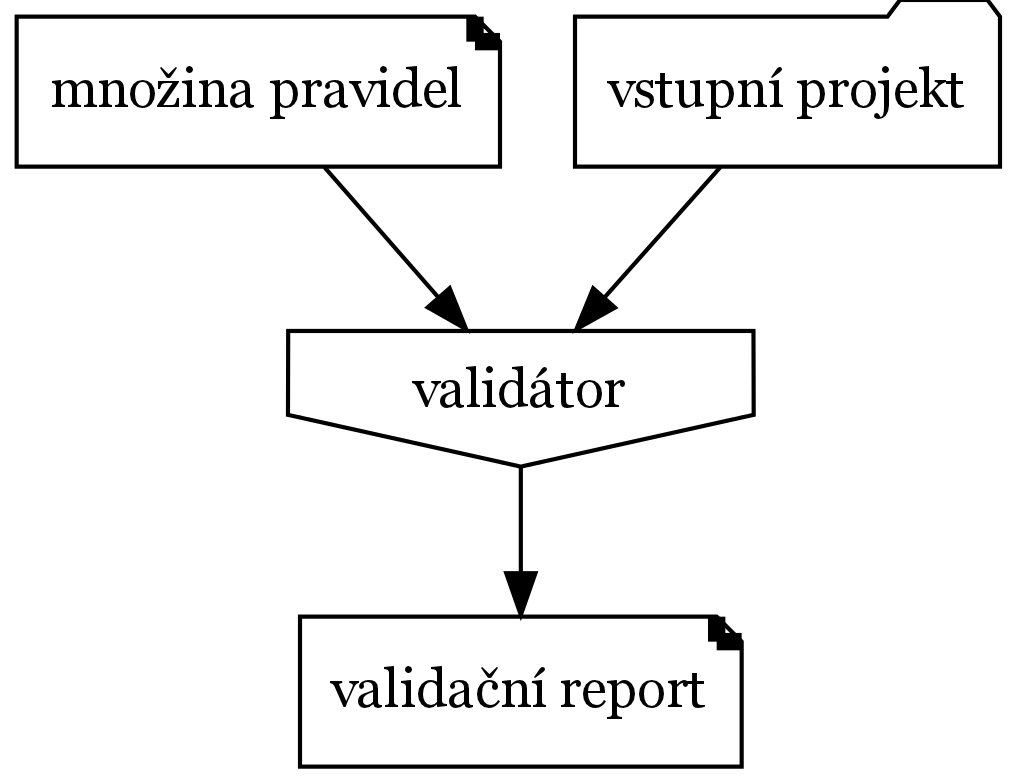
\includegraphics[width=0.5\textwidth]{./graphs/global_structure.png}
  \caption{Struktura systému.\label{requirements-system_structure}}
\end{figure}

Výstupem systému by měl být \emph{validační report}, který vypíše, která pravidla ze vstupního souboru byla porušena. Formát vstupních pravidel a výstupního reportu bude definován dále.

\subsection{Funkční požadavky na výsledný systém}

Na základě obecných požadavků můžeme specifikovat základní funkční požadavky. Požadujeme, aby systém uměl provádět následující funkčnosti:
\begin{itemize}
\item načíst vhodně předzpracovaný projekt realizovaný v jazyce Java a vytvořit vnitřní model pro další analýzu,
\item načíst ze vstupního souboru množinu pravidel v~definovaném formátu,
\item provést validaci načteného modelu pomocí množiny pravidel,
\item vypsat report obsahující informace o~splnění resp. porušení pravidel.
\end{itemize}

\subsection{Nefunkční požadavky na výsledný systém}
Z~nefunkční požadavků je zadáním práce dán požadavek na \emph{rozšiřitelnost}. Systém by mělo být možné rozšířit o~další modely a možnosti specifikace nových/složitějších pravidel nad modely.

\section{Rešerše existujících řešení}
\label{requirements-existing_tools}

V~této sekci se postupně podíváme na různé nástroje, které si kladou za cíl ověřování kvality kódu na různých úrovních. Každý z~těchto nástrojů pojímá kontrolu kvality zdrojového kódu poněkud jiným způsobem. Některé se zabývají \uv{pouhou} analýzou na úrovni jedné kompilační jednotky\footnote{Kompilační jednotka je u~jazyka Java představována jedním \verb-*.java- souborem.}, jiné provádějí strukturální analýzu na úrovni vztahů mezi jednotlivými třídami.

\subsection{CheckStyle}
\emph{CheckStyle} je vývojový nástroj, který si klade za cíl pomoci programátorům psát Java kód, který vyhovuje konkrétním kódovým konvencím \cite{existingtools:checkstyle}. Pracuje na úrovni jednoduchého zpracovávání \verb+*.java+ souborů a kontroluje např. přítomnost \verb+javadoc+ komentářů nad třídami, atributy a metodami, jmenné konvence, maximální povolené počty parametrů, délky řádků, duplicitní kód atd. \cite{existingtools:checkstyle-wiki}. Zvládne i jednodušší testy na zjištění složitosti kódu (podle klíčových slov for, while, atd.). Kódové konvence jsou konfigurovatelné pomocí XML souborů, kde lze vybírat, která předdefinovaná pravidla se budou v~kódu kontrolovat (např. pravidlo \mbox{\uv{AvoidStarImport}} apod.).

\subsection{DP-Miner}
Autoři článku \cite{4273268} a nástroje \emph{DP-Miner} \cite{existingtools:dp-miner} se zabývají výzkumem v~oblasti návrhových vzorů. Ukazuje se, že návrhové vzory jsou velmi důležité a extenzivně využívané ve fázi návrhu software. Při realizaci v~konkrétním zdrojovém kódu se však informace o~návrhových vzorech zpravidla ztrácí. Cílem nástroje \emph{DP-Miner} je objevování návrhových vzorů v~existujících projektech, k~nimž neexistuje vývojová dokumentace. Ve článku \cite{4273268} jsou demonstrovány schopnosti odhalit návrhové vzory na reálných projektech jako např. \emph{JUnit}, \emph{JEdit}, \emph{Java.AWT} a dalších. Pro odhalování vzorů používají autoři matici vztahů mezi třídami analyzovaného systému.

\subsection{FindBugs}
Nástroj \emph{FindBugs} \cite{existingtools:findbugs} vyhledává potenciální zdroje chyb v~Java programech. Vyhledává chyby podle chybových vzorů. Chybové zdroje jsou idiomy, které se ve zdrojových kódech často vyskytují chybně použity. Většinou se jedná o~obtížněji zvládnutelné vlastnosti jazyka, nepochopení rozhraní některého API atd. (Typickým příkladem může být porovnávání objektů \verb+String+ pomocí operátoru \verb+==+.) Pro odhalování chyb je používána statická analýza. \emph{FindBugs} pracuje nad byte kódem (analyzuje zkompilované třídní \verb-*.class- soubory) -- \mbox{je tedy} možné analyzovat i programy, k~nimž nemáme k~dispozici zdrojové kódy. Analýza je mnohdy nepřesná (ne všechny vzory chyb jsou vždy opravdu chybami -- může se jednat o~záměrné použití). Nástroj v~takovém případě chybně vypisuje varování, která neznamenají chybu (falešně pozitivní případy).

\subsection{JDepend}
Podobně jako předchozí nástroj pracuje i \emph{JDepend} \cite{existingtools:jdepend} nad zkompilovanými \verb+*.class+ soubory jazyka Java. Funguje však na jiném principu a na daleko vyšší úrovni. Zabývá se analýzou závislostí mezi třídami a balíčky. Systém poskytuje výpis základních metrik, jako je počet tříd a rozhraní v~balíčcích, počet závislých balíčků (to je zde označováno jako \uv{zodpovědnost} -- čím více tříd na balíčku závisí, tím větší je jeho zodpovědnost). Vesměs se jedná o~metriky založené na počtech elementů v~projektu. Za zmínku stojí odhalování cyklů v~závislostech balíčků.

\subsection{Macker}
Velmi zajímavým nástrojem je \emph{Macker} \cite{existingtools:macker}. Pracuje na strukturální úrovni během kompilace a umožňuje kontrolovat nejrůznější strukturální pravidla. Stejně jako předchozí dva nástroje operuje nad zkompilovanými \verb+*.class+ soubory. Mezi zajímavá pravidla, která je schopen vynutit patří například:

\begin{itemize}
\item \uv{třídy z~UI vrstvy nesmí přímo přistupovat k~objektům v~datové vrstvě nebo používat třídy v~balíčku \verb-java.sql-},
\item \uv{externí systémy nesmí přistupovat k~interním implementačním třídám (které mají sufix 'Impl')},
\item \uv{jeden funkční modul smí přistupovat ke druhému pouze přes jeho API}.
\end{itemize}

Z~uvedených pravidel je patrné, že \emph{Macker} operuje na globální strukturální úrovni a je schopen vynutit dodatečnou kontrolu přístupu (vedle standardních prostředků jazyka Java, kterými jsou modifikátory přístupu).

\subsection{PMD}
Velmi rozšířený nástroj \emph{PMD} \cite{existingtools:pmd} prochází zdrojové kódy jazyka Java a vyhledává potenciální zdroje problémů (srov. s~nástrojem \emph{FindBugs}). Příkladem vyhledávaných vzorů jsou:

\begin{itemize}
\item možné chyby -- prázdné příkazy \emph{try/catch/finally/switch},
\item mrtvý kód -- nepoužité lokální proměnné, parametry a privátní metody\footnote{To je dnes běžné téměř pro všechna nejčastěji používaná IDE pro vývoj v~jazyce Java.},
\item neoptimální kód -- neefektivní využívání tříd String/StringBuffer,
\item příliš komplikované výrazy -- zbytečné \verb+if+ příkazy, cykly \verb+for+, které mohou být realizovány pomocí \verb+while+.
\end{itemize}

Výhodou \emph{PMD} je integrovanost s~velkým množstvím nástrojů (JDeveloper, Eclipse, JEdit, JBuilder, ItelliJ IDEA, Maven, Emacs, a další).

\subsection{QJ-Pro}
Dalším pokročilým nástrojem je \emph{QJ-Pro} \cite{existingtools:qjpro}. Pracuje nad zdrojovými kódy a poskytuje velké množství pravidel, která lze vyhodnocovat. Kromě vynucení běžných kódových konvencí podporuje navíc analýzu nejrůznějších metrik (počet metod na třídu, poměr privátních a public polí, a další.). Existuje integrace do vývojových prostředí -- např. Eclipse IDE a~Borland JBuilder.

\subsection{Soot}
Poněkud odlišným nástrojem je \emph{Soot} \cite{existingtools:soot}. Jedná se o~framework pro optimalizaci Java kódu. Na rozdíl od předchozích zmiňovaných nástrojů, které jsou určeny spíše běžným programátorům, se jedná výzkumný projekt a platformu, na které je možné vyvíjet nástroje pro optimalizaci a analýzu. Nástroj pracuje nad Java byte kódem. Existuje integrace do Eclipse IDE.

\subsection{Squale}
\emph{Squale}\footnote{Uvedený název je odvozen z~úplného názvu \uv{Software QUALity Enhancement}.} \cite{existingtools:squale} je opět zcela jiný pohled na práci se zdrojovými kódy. Nejedná se o~běžný analyzátor kódu (jako téměř všechny předchozí případy) ale spíše o~monitorovací nástroj, který umožní sledovat přehledně metriky zdrojových kódů. Případy užití tohoto nástroje tedy spadají spíše do oblasti managementu (vyhodnocování výkonnosti týmu, kvality jejich kódu atd.).
